% !TeX program = xelatex
\documentclass{article}
\usepackage{kotex}
\usepackage[a4paper,left=3cm, right=3cm, top=2cm, bottom=2cm]{geometry}
\usepackage{amsmath}
\usepackage{graphicx}
\usepackage{caption}
\usepackage{setspace}
\usepackage{xcolor}
\usepackage{titlesec}
\usepackage{amssymb}
\usepackage{tcolorbox}
\usepackage{amsthm}
\usepackage{multirow}
\usepackage{array}
\usepackage{booktabs}
\usepackage{tikz}
\usetikzlibrary{positioning,arrows.meta,calc,shapes.geometric,matrix}
\usepackage{cancel}
\usepackage{pgfplots}
\pgfplotsset{compat=1.18}

\title{8.4 Matrices for General Linear Transformations}
\date{}
\author{}
\setstretch{1.3}

\titleformat{name=\section, numberless}
  {\normalfont\large\bfseries\color{blue}}{}
  {0pt}{}
\geometry{a4paper, margin=1in}

\newcommand{\redheading}[1]{{\vspace{2mm}\noindent\Large\bfseries\color{red!55!black} #1\par}\vspace{2mm}}

\begin{document}
\maketitle

{\itshape\color{blue!45!black}
In this section we show that a general linear transformation from any $n$-dimensional
vector space $V$ to any $m$-dimensional vector space $W$ can be performed using an
appropriate matrix transformation from $R^n$ to $R^m$. This idea is used in computer
computations since computers are well suited for performing matrix computations.\par}

\vspace{2mm}

\redheading{Matrices of Linear Transformations}

Suppose $V$ is $n$-dimensional, $W$ is $m$-dimensional, and $T : V \to W$ is a linear
transformation. Let $B = \{\mathbf{u}_1,\ldots,\mathbf{u}_n\}$ be a basis for $V$ and
$B' = \{\mathbf{v}_1,\ldots,\mathbf{v}_m\}$ a basis for $W$. For each $\mathbf{x} \in V$,
the coordinate vectors $[\mathbf{x}]_B \in R^n$ and $[T(\mathbf{x})]_{B'} \in R^m$ are
related by the following commutative diagram:

\begin{figure}[ht]
\centering
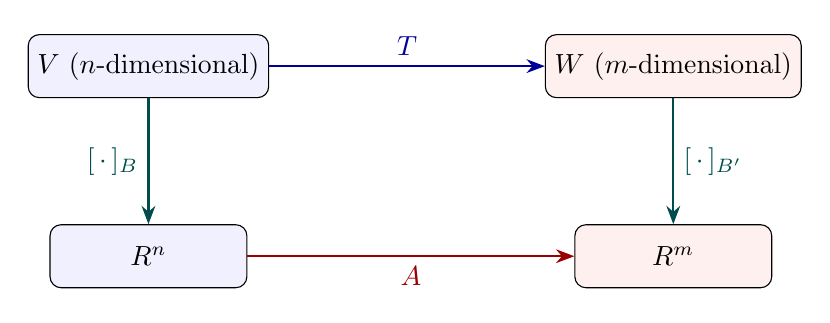
\begin{tikzpicture}[>=Stealth, node distance=1.5cm, auto]
  \node[draw, rounded corners, minimum width=2.5cm, minimum height=0.8cm,
    fill=blue!6] (V) {$V$ ($n$-dimensional)};
  \node[draw, rounded corners, minimum width=2.5cm, minimum height=0.8cm,
    fill=red!6, right=3.5cm of V] (W) {$W$ ($m$-dimensional)};
  \node[draw, rounded corners, minimum width=2.5cm, minimum height=0.8cm,
    fill=blue!6, below=1.6cm of V] (Rn) {$R^n$};
  \node[draw, rounded corners, minimum width=2.5cm, minimum height=0.8cm,
    fill=red!6, below=1.6cm of W] (Rm) {$R^m$};
  \draw[->, thick, blue!60!black] (V) -- node[above]{$T$} (W);
  \draw[->, thick, teal!60!black] (V) -- node[left]{$[\,\cdot\,]_B$} (Rn);
  \draw[->, thick, teal!60!black] (W) -- node[right]{$[\,\cdot\,]_{B'}$} (Rm);
  \draw[->, thick, red!60!black] (Rn) -- node[below]{$A$} (Rm);
\end{tikzpicture}
\caption*{FIGURE 8.4.1}
\end{figure}

Our goal is to find an $m \times n$ matrix $A$ such that
\begin{equation}
  A[\mathbf{x}]_B = [T(\mathbf{x})]_{B'} \tag{1}
\end{equation}
for all $\mathbf{x} \in V$. With such an $A$, computing $T(\mathbf{x})$ can be done
\emph{indirectly} in three steps:

\begin{tcolorbox}[colback=blue!4, colframe=blue!55!black,
  title={\textbf{Finding $T(\mathbf{x})$ Indirectly}}, boxrule=0.5mm, arc=3mm]
\textbf{Step 1.} Compute the coordinate vector $[\mathbf{x}]_B$.\\
\textbf{Step 2.} Multiply $[\mathbf{x}]_B$ on the left by $A$ to produce $[T(\mathbf{x})]_{B'}$.\\
\textbf{Step 3.} Reconstruct $T(\mathbf{x})$ from its coordinate vector $[T(\mathbf{x})]_{B'}$.
\end{tcolorbox}

\begin{figure}[ht]
\centering
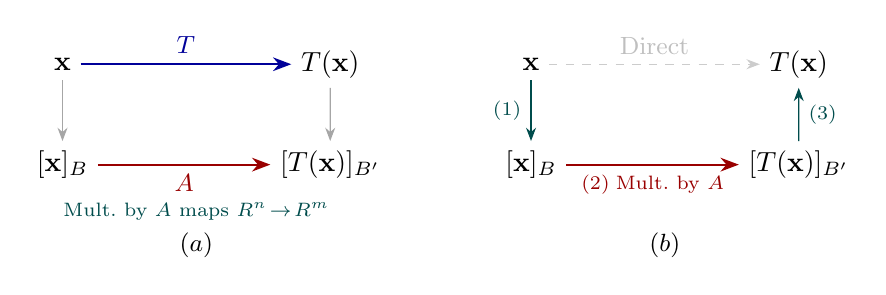
\begin{tikzpicture}[>=Stealth, scale=0.85]
  %--- Panel (a): direct vs indirect ---
  \begin{scope}[xshift=0cm]
    \node (x1) at (0,1.5) {$\mathbf{x}$};
    \node (Tx1) at (4,1.5) {$T(\mathbf{x})$};
    \node (xb1) at (0,0) {$[\mathbf{x}]_B$};
    \node (Txb1) at (4,0) {$[T(\mathbf{x})]_{B'}$};
    \draw[->, blue!60!black, thick] (x1) -- node[above,font=\small]{$T$} (Tx1);
    \draw[->, gray!70] (x1) -- node[left, font=\scriptsize]{} (xb1);
    \draw[->, gray!70] (Tx1) -- (Txb1);
    \draw[->, red!60!black, thick] (xb1) -- node[below,font=\small]{$A$} (Txb1);
    \node[font=\scriptsize, teal!60!black] at (2,-0.7) {Mult.\ by $A$ maps $R^n\!\to\!R^m$};
    \node[font=\small] at (2,-1.2) {$(a)$};
  \end{scope}
  %--- Panel (b): 3-step ---
  \begin{scope}[xshift=7cm]
    \node (x2) at (0,1.5) {$\mathbf{x}$};
    \node (Tx2) at (4,1.5) {$T(\mathbf{x})$};
    \node (xb2) at (0,0) {$[\mathbf{x}]_B$};
    \node (Txb2) at (4,0) {$[T(\mathbf{x})]_{B'}$};
    \draw[->, gray!40, dashed] (x2) -- node[above,font=\small,gray!50]{Direct} (Tx2);
    \draw[->, teal!60!black] (x2) -- node[left,font=\scriptsize]{$(1)$} (xb2);
    \draw[->, teal!60!black] (Txb2) -- node[right,font=\scriptsize]{$(3)$} (Tx2);
    \draw[->, red!60!black, thick] (xb2) -- node[below,font=\scriptsize]{$(2)$\;Mult.\ by $A$} (Txb2);
    \node[font=\small] at (2,-1.2) {$(b)$};
  \end{scope}
\end{tikzpicture}
\caption*{FIGURE 8.4.2}
\end{figure}

To find $A$, note that Equation~(1) must hold for each basis vector $\mathbf{u}_i$ in $B$.
Since $[\mathbf{u}_i]_B = \mathbf{e}_i$ (the $i$-th standard basis vector in $R^n$),
multiplying $A$ by $\mathbf{e}_i$ picks out the $i$-th column of $A$, which must equal
$[T(\mathbf{u}_i)]_{B'}$. Thus the successive columns of $A$ are the coordinate vectors of
$T(\mathbf{u}_1), T(\mathbf{u}_2), \ldots, T(\mathbf{u}_n)$ with respect to $B'$. We call
this matrix the \textbf{matrix for $T$ relative to the bases $B$ and $B'$}, denoted
$[T]_{B',B}$:
\begin{equation}
  \boxed{[T]_{B',B} = \bigl[\,[T(\mathbf{u}_1)]_{B'}\;\big|\;[T(\mathbf{u}_2)]_{B'}\;\big|\;
  \cdots\;\big|\;[T(\mathbf{u}_n)]_{B'}\,\bigr]} \tag{4}
\end{equation}
and this matrix satisfies
\begin{equation}
  \boxed{[T]_{B',B}[\mathbf{x}]_B = [T(\mathbf{x})]_{B'}} \tag{5}
\end{equation}

\textit{Remark.} In the notation $[T]_{B',B}$, the \emph{right} subscript $B$ is the
basis for the \emph{domain} of $T$, and the \emph{left} subscript $B'$ is the basis for
the \emph{image space}. Observe how $B$ "cancels out" in Formula~(5): $[T]_{B',\cancel{B}}
[\mathbf{x}]_{\cancel{B}} = [T(\mathbf{x})]_{B'}$.

When $T_C : R^n \to R^m$ is multiplication by $C$ and $S$, $S'$ are the standard bases
for $R^n$ and $R^m$, then
\begin{equation}
  [T_C]_{S',S} = C \tag{6}
\end{equation}

\subsection*{EXAMPLE 1 | Matrix for a Linear Transformation}

Let $T : P_1 \to P_2$ be defined by $T(p(x)) = xp(x)$. Find the matrix for $T$ with
respect to the standard bases $B = \{\mathbf{u}_1, \mathbf{u}_2\} = \{1, x\}$ and
$B' = \{\mathbf{v}_1, \mathbf{v}_2, \mathbf{v}_3\} = \{1, x, x^2\}$.

\textbf{SOLUTION:} Compute:
\[
  T(\mathbf{u}_1) = T(1) = x, \qquad T(\mathbf{u}_2) = T(x) = x^2
\]
Their coordinate vectors relative to $B'$ are
\[
  [T(\mathbf{u}_1)]_{B'} = \begin{bmatrix}0\\1\\0\end{bmatrix}, \qquad
  [T(\mathbf{u}_2)]_{B'} = \begin{bmatrix}0\\0\\1\end{bmatrix}
\]
so by Formula~(4),
\[
  [T]_{B',B} = \begin{bmatrix}0&0\\1&0\\0&1\end{bmatrix}
\]

\subsection*{EXAMPLE 2 | The Three-Step Procedure}

Use the matrix from Example~1 to compute $T(a+bx) = x(a+bx) = ax+bx^2$.

\textbf{SOLUTION:}
\textbf{Step 1.} $[\mathbf{x}]_B = \begin{bmatrix}a\\b\end{bmatrix}$.

\textbf{Step 2.} $[T]_{B',B}[\mathbf{x}]_B = \begin{bmatrix}0&0\\1&0\\0&1\end{bmatrix}
\begin{bmatrix}a\\b\end{bmatrix} = \begin{bmatrix}0\\a\\b\end{bmatrix} = [T(\mathbf{x})]_{B'}$.

\textbf{Step 3.} $T(a+bx) = 0\cdot 1 + a\cdot x + b\cdot x^2 = ax + bx^2$. $\checkmark$

\subsection*{EXAMPLE 3 | Matrix for a Linear Transformation}

Let $T : R^2 \to R^3$ be defined by
\[
  T\!\left(\begin{bmatrix}x_1\\x_2\end{bmatrix}\right)
  = \begin{bmatrix}x_2\\-5x_1+13x_2\\-7x_1+16x_2\end{bmatrix}
  = \begin{bmatrix}0&1\\-5&13\\-7&16\end{bmatrix}\begin{bmatrix}x_1\\x_2\end{bmatrix}
\]
Find $[T]_{B',B}$ relative to the bases $B = \{\mathbf{u}_1, \mathbf{u}_2\}$ for $R^2$
and $B' = \{\mathbf{v}_1, \mathbf{v}_2, \mathbf{v}_3\}$ for $R^3$, where
\[
  \mathbf{u}_1 = \begin{bmatrix}3\\1\end{bmatrix},\quad
  \mathbf{u}_2 = \begin{bmatrix}5\\2\end{bmatrix};\qquad
  \mathbf{v}_1 = \begin{bmatrix}1\\0\\-1\end{bmatrix},\quad
  \mathbf{v}_2 = \begin{bmatrix}-1\\2\\2\end{bmatrix},\quad
  \mathbf{v}_3 = \begin{bmatrix}0\\1\\2\end{bmatrix}
\]

\textbf{SOLUTION:} First compute:
\[
  T(\mathbf{u}_1) = \begin{bmatrix}1\\-2\\-5\end{bmatrix}, \qquad
  T(\mathbf{u}_2) = \begin{bmatrix}2\\1\\-3\end{bmatrix}
\]
Expressing these as linear combinations of $\mathbf{v}_1, \mathbf{v}_2, \mathbf{v}_3$
(verify):
\[
  T(\mathbf{u}_1) = \mathbf{v}_1 - 2\mathbf{v}_3, \qquad
  T(\mathbf{u}_2) = 3\mathbf{v}_1 + \mathbf{v}_2 - \mathbf{v}_3
\]
so
\[
  [T(\mathbf{u}_1)]_{B'} = \begin{bmatrix}1\\0\\-2\end{bmatrix}, \qquad
  [T(\mathbf{u}_2)]_{B'} = \begin{bmatrix}3\\1\\-1\end{bmatrix}
\]
and
\[
  [T]_{B',B} = \begin{bmatrix}1&3\\0&1\\-2&-1\end{bmatrix}
\]

\textit{Remark.} A fixed linear transformation has \emph{multiple} matrix representations
depending on the bases. Here
\[
  [T]_{S',S} = \begin{bmatrix}0&1\\-5&13\\-7&16\end{bmatrix} \qquad\text{and}\qquad
  [T]_{B',B} = \begin{bmatrix}1&3\\0&1\\-2&-1\end{bmatrix}
\]
both represent $T$: the first relative to the standard bases $S$ and $S'$, the second
relative to $B$ and $B'$.

\vspace{2mm}
\redheading{Matrices of Linear Operators}

When $V = W$ (so $T : V \to V$ is a linear \emph{operator}), we take $B = B'$. The
resulting matrix is called the \textbf{matrix for $T$ relative to the basis $B$}, denoted
$[T]_B$. Formulas (4) and (5) specialize to
\begin{equation}
  \boxed{[T]_B = \bigl[\,[T(\mathbf{u}_1)]_B\;\big|\;[T(\mathbf{u}_2)]_B\;\big|\;
  \cdots\;\big|\;[T(\mathbf{u}_n)]_B\,\bigr]} \tag{7}
\end{equation}
\begin{equation}
  \boxed{[T]_B[\mathbf{x}]_B = [T(\mathbf{x})]_B} \tag{8}
\end{equation}
For matrix operators $T_A : R^n \to R^n$ with $B$ the standard basis, Formula~(7)
reduces to
\begin{equation}
  [T_A]_B = A \tag{9}
\end{equation}

\redheading{Matrices of Identity Operators}

\subsection*{EXAMPLE 4 | Matrices of Identity Operators}

If $B = \{\mathbf{u}_1, \ldots, \mathbf{u}_n\}$ is a basis for $V$ and $I : V \to V$ is
the identity operator, then $I(\mathbf{u}_i) = \mathbf{u}_i$, so $[I(\mathbf{u}_i)]_B =
\mathbf{e}_i$. Thus $[I]_B = I$ (the $n\times n$ identity matrix) for every basis $B$.

\subsection*{EXAMPLE 5 | Linear Operator on $P_2$}

Let $T : P_2 \to P_2$ be the linear operator defined by $T(p(x)) = p(3x-5)$, that is,
$T(c_0+c_1x+c_2x^2) = c_0+c_1(3x-5)+c_2(3x-5)^2$.

\textbf{(a)} Find $[T]_B$ relative to the basis $B = \{1, x, x^2\}$.

\textbf{(b)} Use the indirect procedure to compute $T(1+2x+3x^2)$.

\textbf{(c)} Check part~(b) by direct computation.

\textbf{SOLUTION (a).} Compute the images of the basis vectors:
\[
  T(1) = 1,\quad T(x) = 3x-5,\quad T(x^2) = (3x-5)^2 = 9x^2-30x+25
\]
Their coordinate vectors relative to $B$:
\[
  [T(1)]_B = \begin{bmatrix}1\\0\\0\end{bmatrix},\quad
  [T(x)]_B = \begin{bmatrix}-5\\3\\0\end{bmatrix},\quad
  [T(x^2)]_B = \begin{bmatrix}25\\-30\\9\end{bmatrix}
\]
so
\[
  [T]_B = \begin{bmatrix}1&-5&25\\0&3&-30\\0&0&9\end{bmatrix}
\]

\textbf{SOLUTION (b).} Let $\mathbf{p} = 1+2x+3x^2$.

\textbf{Step 1.} $[\mathbf{p}]_B = \begin{bmatrix}1\\2\\3\end{bmatrix}$.

\textbf{Step 2.} $[T]_B[\mathbf{p}]_B = \begin{bmatrix}1&-5&25\\0&3&-30\\0&0&9\end{bmatrix}
\begin{bmatrix}1\\2\\3\end{bmatrix} = \begin{bmatrix}66\\-84\\27\end{bmatrix} = [T(\mathbf{p})]_B$.

\textbf{Step 3.} $T(1+2x+3x^2) = 66 - 84x + 27x^2$.

\textbf{SOLUTION (c).} Direct computation:
\begin{align*}
  T(1+2x+3x^2) &= 1 + 2(3x-5) + 3(3x-5)^2\\
  &= 1 + 6x-10 + 3(9x^2-30x+25) = 66 - 84x + 27x^2 \quad\checkmark
\end{align*}

\vspace{2mm}
\redheading{Matrices of Compositions and Inverse Transformations}

\begin{tcolorbox}[colback=red!4, colframe=red!60!black,
  title={\textbf{Theorem 8.4.1}}, boxrule=0.5mm, arc=3mm]
If $T_1 : U \to V$ and $T_2 : V \to W$ are linear transformations with bases $B$, $B''$,
$B'$ for $U$, $V$, $W$ respectively, then
\begin{equation}
  [T_2 \circ T_1]_{B',B} = [T_2]_{B',B''}[T_1]_{B'',B} \tag{10}
\end{equation}
\end{tcolorbox}

\begin{tcolorbox}[colback=red!4, colframe=red!60!black,
  title={\textbf{Theorem 8.4.2}}, boxrule=0.5mm, arc=3mm]
If $T : V \to V$ is a linear operator and $B$ is a basis for $V$, then the following
are equivalent:
\begin{enumerate}
  \item[(a)] $T$ is one-to-one.
  \item[(b)] $[T]_B$ is invertible.
\end{enumerate}
Moreover, when these conditions hold,
\begin{equation}
  [T^{-1}]_B = [T]_B^{-1} \tag{11}
\end{equation}
\end{tcolorbox}

\textit{Remark.} Observe how the interior subscript $B''$ in Formula~(10) "cancels," leaving
only the bases for the domain and image. This cancellation extends to three transformations:
if $T_1: U\to V$, $T_2: V\to W$, $T_3: W\to Y$, then
\begin{equation}
  [T_3 \circ T_2 \circ T_1]_{B',B}
  = [T_3]_{B',B'''}[T_2]_{B''',B''}[T_1]_{B'',B} \tag{12}
\end{equation}

\begin{figure}[ht]
\centering
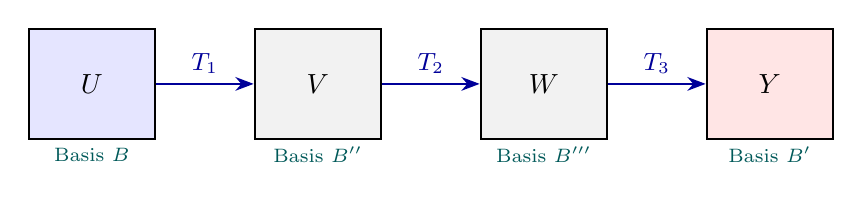
\begin{tikzpicture}[>=Stealth, scale=0.82]
  \node[draw, thick, fill=blue!10, minimum width=1.6cm, minimum height=1.4cm] (U) at (0,0) {$U$};
  \node[font=\scriptsize, teal!70!black] at (0,-1.1) {Basis $B$};
  \node[draw, thick, fill=gray!10, minimum width=1.6cm, minimum height=1.4cm] (V) at (3.5,0) {$V$};
  \node[font=\scriptsize, teal!70!black] at (3.5,-1.1) {Basis $B''$};
  \node[draw, thick, fill=gray!10, minimum width=1.6cm, minimum height=1.4cm] (W) at (7,0) {$W$};
  \node[font=\scriptsize, teal!70!black] at (7,-1.1) {Basis $B'''$};
  \node[draw, thick, fill=red!10, minimum width=1.6cm, minimum height=1.4cm] (Y) at (10.5,0) {$Y$};
  \node[font=\scriptsize, teal!70!black] at (10.5,-1.1) {Basis $B'$};
  \draw[->, blue!60!black, thick] (U) -- node[above, font=\small]{$T_1$} (V);
  \draw[->, blue!60!black, thick] (V) -- node[above, font=\small]{$T_2$} (W);
  \draw[->, blue!60!black, thick] (W) -- node[above, font=\small]{$T_3$} (Y);
\end{tikzpicture}
\caption*{FIGURE 8.4.6}
\end{figure}

\subsection*{EXAMPLE 6 | Composition}

Let $T_1 : P_1 \to P_2$ be defined by $T_1(p(x)) = xp(x)$ and
$T_2 : P_2 \to P_2$ by $T_2(p(x)) = p(3x-5)$.
The composition $(T_2 \circ T_1) : P_1 \to P_2$ is
\[
  (T_2 \circ T_1)(p(x)) = T_2(xp(x)) = (3x-5)p(3x-5)
\]
so for $p(x) = c_0 + c_1 x$,
\[
  (T_2 \circ T_1)(c_0+c_1 x) = c_0(3x-5) + c_1(3x-5)^2 \tag{13}
\]
In Theorem~8.4.1, $P_2$ plays both the role of $V$ and $W$, so $B'' = B' = \{1,x,x^2\}$.
Formula~(10) simplifies to
\[
  [T_2\circ T_1]_{B',B} = [T_2]_{B'}[T_1]_{B',B} \tag{14}
\]
Using $[T_1]_{B',B}$ from Example~1 and $[T_2]_{B'}$ from Example~5:
\begin{equation}
  [T_2\circ T_1]_{B',B}
  = \begin{bmatrix}1&-5&25\\0&3&-30\\0&0&9\end{bmatrix}
    \begin{bmatrix}0&0\\1&0\\0&1\end{bmatrix}
  = \begin{bmatrix}-5&25\\3&-30\\0&9\end{bmatrix} \tag{15}
\end{equation}
\textbf{Verification.} From (13): $(T_2\circ T_1)(1) = 3x-5$ and $(T_2\circ T_1)(x) = (3x-5)^2 = 9x^2-30x+25$.
Their coordinate vectors w.r.t.\ $B'$ are $[-5;3;0]$ and $[25;-30;9]$, giving
$[T_2\circ T_1]_{B',B} = \begin{bmatrix}-5&25\\3&-30\\0&9\end{bmatrix}$, which agrees with~(15). $\checkmark$

\vspace{3mm}
\noindent\rule{\linewidth}{0.5pt}

\section*{Exercise Set 8.4}

\noindent\textit{In Exercises 1--8, find the matrix for the linear transformation relative
to the indicated bases.}

\begin{enumerate}
  \item Let $T : P_2 \to P_3$ be defined by $T(p(x)) = xp(x)$.\\
        \textbf{a.} Find the matrix for $T$ relative to the standard bases
        $B = \{\mathbf{u}_1,\mathbf{u}_2,\mathbf{u}_3\} = \{1,x,x^2\}$ and
        $B' = \{\mathbf{v}_1,\mathbf{v}_2,\mathbf{v}_3,\mathbf{v}_4\} = \{1,x,x^2,x^3\}$.\\
        \textbf{b.} Verify that $[T]_{B',B}$ satisfies Formula~(5) for every
        $\mathbf{x} = c_0+c_1x+c_2x^2$ in $P_2$.

  \item[3.] Let $T : P_2 \to P_2$ be the linear operator defined by
        $T(a_0+a_1x+a_2x^2) = a_0+a_1(x-1)+a_2(x-1)^2$.\\
        \textbf{a.} Find the matrix for $T$ relative to the standard basis $B = \{1,x,x^2\}$.\\
        \textbf{b.} Verify that $[T]_B$ satisfies Formula~(8) for every
        $\mathbf{x} = a_0+a_1x+a_2x^2$ in $P_2$.

  \item[4.] Let $T : R^2 \to R^2$ be the linear operator defined by
        $T\!\left(\begin{bmatrix}x_1\\x_2\end{bmatrix}\right)
        = \begin{bmatrix}x_1-x_2\\x_1+x_2\end{bmatrix}$,
        and let $B = \{\mathbf{u}_1,\mathbf{u}_2\}$ where
        $\mathbf{u}_1 = \begin{bmatrix}1\\1\end{bmatrix}$,
        $\mathbf{u}_2 = \begin{bmatrix}-1\\0\end{bmatrix}$.\\
        \textbf{a.} Find $[T]_B$.\\
        \textbf{b.} Verify that $[T]_B$ satisfies Formula~(8) for every vector $\mathbf{x}$ in $R^2$.

  \item[7.] Let $T : P_2 \to P_2$ be the linear operator $T(p(x)) = p(2x+1)$, that is,
        $T(c_0+c_1x+c_2x^2) = c_0+c_1(2x+1)+c_2(2x+1)^2$.\\
        \textbf{a.} Find $[T]_B$ with respect to the basis $B = \{1,x,x^2\}$.\\
        \textbf{b.} Use the three-step procedure to compute $T(2-3x+4x^2)$.\\
        \textbf{c.} Check the result in (b) by computing $T(2-3x+4x^2)$ directly.

\end{enumerate}

\noindent\textit{In Exercises 9--11, the matrix $A$ for $T$ relative to a given basis is
provided; find $T$ explicitly.}

\begin{enumerate}
  \item[9.] Let $\mathbf{v}_1 = \begin{bmatrix}1\\3\end{bmatrix}$ and
        $\mathbf{v}_2 = \begin{bmatrix}-1\\4\end{bmatrix}$, and let
        $A = \begin{bmatrix}1&3\\-2&5\end{bmatrix}$ be the matrix for
        $T : R^2 \to R^2$ relative to $B = \{\mathbf{v}_1,\mathbf{v}_2\}$.\\
        \textbf{a.} Find $[T(\mathbf{v}_1)]_B$ and $[T(\mathbf{v}_2)]_B$.\\
        \textbf{b.} Find $T(\mathbf{v}_1)$ and $T(\mathbf{v}_2)$.\\
        \textbf{c.} Find a formula for $T\!\left(\begin{bmatrix}x_1\\x_2\end{bmatrix}\right)$.\\
        \textbf{d.} Use the formula in (c) to compute $T\!\left(\begin{bmatrix}1\\1\end{bmatrix}\right)$.

  \item[11.] Let $A = \begin{bmatrix}1&3&-1\\2&0&5\\6&-2&4\end{bmatrix}$ be the matrix for
        $T : P_2 \to P_2$ with respect to the basis $B = \{\mathbf{v}_1,\mathbf{v}_2,\mathbf{v}_3\}$,
        where $\mathbf{v}_1 = 3x+3x^2$, $\mathbf{v}_2 = -1+3x+2x^2$, $\mathbf{v}_3 = 3+7x+2x^2$.\\
        \textbf{a.} Find $[T(\mathbf{v}_1)]_B$, $[T(\mathbf{v}_2)]_B$, and $[T(\mathbf{v}_3)]_B$.\\
        \textbf{b.} Find $T(\mathbf{v}_1)$, $T(\mathbf{v}_2)$, and $T(\mathbf{v}_3)$.\\
        \textbf{c.} Find a formula for $T(a_0+a_1x+a_2x^2)$.\\
        \textbf{d.} Use the formula in (c) to compute $T(1+x^2)$.

\end{enumerate}

\begin{enumerate}
  \item[12.] Let $T_1 : P_1 \to P_2$ be defined by $T_1(p(x)) = xp(x)$ and let
        $T_2 : P_2 \to P_2$ be defined by $T_2(p(x)) = p(2x+1)$.
        Let $B = \{1,x\}$ and $B' = \{1,x,x^2\}$ be the standard bases for $P_1$ and $P_2$.\\
        \textbf{a.} Find $[T_2\circ T_1]_{B',B}$, $[T_2]_{B'}$, and $[T_1]_{B',B}$.\\
        \textbf{b.} State a formula relating the matrices in part~(a).\\
        \textbf{c.} Verify that the matrices in part~(a) satisfy the formula in~(b).

  \item[14.] Let $B = \{\mathbf{v}_1,\mathbf{v}_2,\mathbf{v}_3,\mathbf{v}_4\}$ be a basis
        for a vector space $V$. Find the matrix with respect to $B$ for the linear operator
        $T : V \to V$ defined by
        $T(\mathbf{v}_1) = \mathbf{v}_2$, $T(\mathbf{v}_2) = \mathbf{v}_3$,
        $T(\mathbf{v}_3) = \mathbf{v}_4$, $T(\mathbf{v}_4) = \mathbf{v}_1$.

  \item[17.] \textit{(Calculus required)} Let $D : P_2 \to P_2$ be the differentiation
        operator $D(\mathbf{p}) = p'(x)$.\\
        \textbf{a.} Find the matrix for $D$ relative to the basis
        $B = \{p_1, p_2, p_3\}$ where $p_1=1$, $p_2=x$, $p_3=x^2$.\\
        \textbf{b.} Use the matrix in (a) to compute $D(6-6x+24x^2)$.

  \item[21.] In each part, fill in the missing subscript.\\
        \textbf{a.} $[T_2\circ T_1]_{B',B} = [T_2]_{\phantom{B',B''}} [T_1]_{B'',B}$\\
        \textbf{b.} $[T_3\circ T_2\circ T_1]_{B',B} = [T_3]_{\phantom{B',B'''}}\,
        [T_2]_{B''',B''}\,[T_1]_{B'',B}$

\end{enumerate}

\noindent\textit{Working with Proofs}

\begin{enumerate}
  \item[22.] Prove: if $T : V \to W$ is the zero transformation, then the matrix for $T$
        with respect to any bases for $V$ and $W$ is a zero matrix.

  \item[23.] Prove: if $B$ and $B'$ are the standard bases for $R^n$ and $R^m$
        respectively, then the matrix for a linear transformation $T : R^n \to R^m$
        relative to $B$ and $B'$ is the standard matrix for $T$.

\end{enumerate}

\end{document}
